\chapter{Evaluation}
\label{ch:Evaluation}

To evaluate the performance of Intelligent History, 
we conducted a controlled laboratory study to gather data from software developers as they answer questions
requiring them to explore commit histories and obtain code rationale information 
about two Java classes from the Apache Kafka repository.
Participants answered a set of questions without Intelligent History,
followed by a different second set of questions with Intelligent History.
On completion of the questions, we then followed with a semi-structured interview
to gather insight on the participants' experiences with examining commits and issues
and their impressions of Intelligent History.
\rev{Our study investigates} the following research questions:

\begin{itemize}[leftmargin=*]
    \item[] \RQ{1}{\rev{Does Intelligent History accurately identify the commits that software developers want to examine?}} 
    \rev{We ask this research question to assess the performance of the underlying approach 
    used in Intelligent History's commit highlighting feature (\feature{1}) \textit{Highlight Important Changes}.}

    \item[] \RQ{2}{Does highlighting important commits help software developers explore a file’s revision history more efficiently?}
    \rev{We propose this research question to evaluate the contexts in which commit highlighting can help software developers
    investigate a commit history more efficiently.}

    \item[] \RQ{3}{How useful is direct integration of issue information in the IDE for helping a developer search for code rationale information?}
    \rev{This research question seeks to gauge the utility of (\feature{3}) \textit{Show Jira Metadata} as
    an implementation of co-presenting issue information and commits in the \entity{IDE}.}
\end{itemize}

We describe the method we designed to address these research questions in detail in \autoref{sec:Method}.
We present the results of our analysis and answer the research questions in \autoref{sec:Results}.

%%%%%%%%%%%%%%%%%%%%%%%%%%%%%%%%%%%%%%%%%%%%%%%%%%%%%%%%%%%%%%%%%%%%%%
\section{Method}
\label{sec:Method}

\rev{We conduct a controlled laboratory study in which participants are
asked to investigate the history of two files: one with the built-in
capabilities of IntelliJ and the other using Intelligent History.}
For the first part, the controlled experiment with an observer allows us to obtain a real-time 
portrayal of how the participants explore and interact with commit history,
and how the presence of Intelligent History influences the participants'
examination of commits to obtain answers to code rationale questions \cite{shull_guide_2007}.
For the second part, the semi-structured interview format allows us to maintain a focused discussion 
while also eliciting interesting responses and reasoning from participants \cite{shull_guide_2007}.
The briefing for the study and the setup instructions can be found in Appendix \ref{sec:Briefing-and-Setup}.

The experiment involved having participants explore the commit history of two Java classes 
from the open-source Apache Kafka project in the IntelliJ IDEA \entity{IDE} 
to find answers to questions related to motivation and rationale behind changes in the classes.
Apache Kafka is an event streaming platform used to collect, process, and store streaming event data.
We chose to use Apache Kafka because the project's contribution guidelines mandates that
each commit must be associated with a Jira issue and the commit's message 
must be prefixed with the issue \entity{ID}, of the form \issue{KAFKA-XXXX}, 
where \issue{XXXX} is a series of numbers for uniquely identifying an issue.
The practice excludes minor commits or hotfixes, 
which are instead prefixed with \issue{MINOR} or \issue{HOTFIX} respectively.
This convention in Apache Kafka will allow the participant to exercise all of the features of Intelligent History
as meaningful commits will generally be associated with a Jira issue in the Apache Kafka project.

Moreover, Apache Kafka also has a practice of maintaing Kafka Improvement Proposals (\entity{KIP}s),
which are documents intended to capture the thought process behind major features introduced 
and changes that impact the public Kafka \entity{API}s.
Commits in the Apache Kafka repository that include changes that are part of \entity{KIP}s will
reference them in their commit messages.
\entity{KIP}s typically have a section titled ``Motivation,''
which can help participants since our experiment will use the commit history 
in Apache Kafka will involve asking the participants to find code rationale information.

The first part of laboratory session consists of 
asking the participants questions about two Java classes from Apache Kafka.
The questions are presented as A1, A2, B1, and B2 in \autoref{tab:Question-Sets}.
Questions A1 and A2 are from set A, while questions B1 and B2 are from set B.
Set A asks about the \class{Topology} class from Apache Kafka and 
set B asks about the \class{StreamsBuilder} class from Apache Kafka.
The \class{Topology} class for set A contains 22 commits and the \class{StreamsBuilder} class for set B contains 45 commits.
The questions are not timed and participants we allow participants to explore the commit history and read Jira issues at their own pace.
We limit the number of questions to two questions per class based on the number of commits in each class' commit history and 
to constrain the duration of the study as a laboratory experiment to a reasonable amount of time.

All questions will require \rev{a} participant to explore and locate particular commits or changes 
from a Java class' commit history to try to find code rationale information that can
help them formulate an answer to each question.
For each question, we expect the participant to inspect \rev{commit messages},
diffs, and any relevant Jira issues to be able to answer the questions.
\rev{For instance, question A2 asks a participant to identify the reasoning
behind why the \class{Topology} class in its present state has multiple overloaded methods called \code{addSink}.
To answer A2, a participant might examine the very first commit in the file to see
whether the \code{addSink} method was initially overloaded and whether the commit contains any motivational information
about the overloads. 
The first commit in the file's commit history has the following title:

\begin{center}
  \jira{KAFKA-5670}{(KIP-120) Add Topology and deprecate TopologyBuilder} (\commit{1844bf2b}).
\end{center}

Code rationale information from the commit \commit{1844bf2b} alone is unavailable as the commit message only 
contains the names of the commit author and code reviewers.
Visiting the referenced Jira issue \issue{KAFKA-5670} yields no further insight due to issue description being blank.
As the commit title references \issue{KIP-120}, a Kafka Improvement Proposal, 
we allow the participant to view this document as part of Apache Kafka's artifacts.
The participant may find that they understand the \class{Topology} class
is a refactoring of a deprecated class but information about the structure of the class
in terms of the overloaded methods is absent.

On further inspecting the diff in \commit{1844bf2b},
the participant may notice that the initial commit does not contain all of the present
\code{addSink} overloads in the class.
The participant might strategize by searching for a commit that introduced further \code{addSink} method overloads 
later in the commit history to be able to find the intent behind the decision.
We do not expect participants to be able to identify \rev{the relevance of this commit to the question} 
based on the commit message title alone.
The participant could examine the diffs of commits
that were made after the first commit in the \class{StreamsBuilder} commit history 
that introduced an initial set of overloaded \code{addSink} methods.
Using this strategy, the participant should eventually locate the correct commit,
which is \commit{f33e9a34} with the following commit message title:

\begin{center}
  \jira{KAFKA-4936:}{Add dynamic routing in Streams (\#5018)}.
\end{center}

Upon accessing \issue{KAFKA-4936}, the participant will see the following description in the issue:

\begin{quote}
  \textsf{
    Currently, all used output topics must be know beforehand, and thus, it's not possible to send output records to topic in a dynamic fashion.
    There have been couple of request for this feature and we should consider adding it.
    There are many open questions however, with regard to topic creation and configuration (replication factor, number of partitions) etc.
  }
\end{quote}

The issue also contains a \entity{URL} link to \issue{KIP-303},
which the participant might visit for further information.
Using information from the issue and optionally, the \entity{KIP}, 
the participant should be able to learn and provide an answer indicating that
the overloads relate to a Kafka topology's sink node and the addition of overloads
supports functionality for sending output records dynamically at the topic level in Apache Kafka.}

\begin{table}[h]
  \caption{
    The question sets used in the laboratory study. 
    Set A pertains to the \class{Topology} class (22 commits) and set B relates to the \class{StreamsBuilder} class (45 commits).
  }
  \centering
  \resizebox{\columnwidth}{!}{%
    \begin{tabular}{@{}c|c|ll@{}}
      \toprule
      Class                           & Set                & \multicolumn{2}{c}{Question}                                                                                                                                                                                                                                                                                                                                      \\ \midrule
      \multirow{2}{*}{\class{Topology}}       & \multirow{2}{*}{A} & \multicolumn{1}{l|}{A1} & \begin{tabular}[c]{@{}l@{}}Can you describe the motivation behind why the\\ code segment on lines 717 to 722 was introduced and the\\ benefit to the user of the Kafka \entity{API}?\end{tabular}                                                                                                                                                \\ \cmidrule(l){3-4} 
                                      &                    & \multicolumn{1}{l|}{A2} & \begin{tabular}[c]{@{}l@{}}There are several overloaded methods called \code{addSink} \\ in this class. \\ Can you describe in what context\\ were these overloaded methods introduced to this class?\end{tabular}                                                                                                                             \\ \midrule
      \multirow{2}{*}{\class{StreamsBuilder}} & \multirow{2}{*}{B} & \multicolumn{1}{l|}{B1} & \begin{tabular}[c]{@{}l@{}}Can you find two commits that introduced changes to\\ improve some functionality in this class and justify why\\ you chose them? \\ The changes can not be cosmetic such as removing \\ repeated words, removing deprecated code,\\ or adding/modifying/removing documentation \\ and comments.\end{tabular} \\ \cmidrule(l){3-4} 
                                      &                    & \multicolumn{1}{l|}{B2} & \begin{tabular}[c]{@{}l@{}}Why is the build method in this class overloaded?\\ Specifically, why was the overloaded \code{build} method in\\ lines 623 to 630 introduced?\end{tabular}                                                                                                                                                         \\ \bottomrule
    \end{tabular}
  }%
  \label{tab:Question-Sets}
\end{table}

We created two different sets, A and B, to facilitate our observation
of how a participant investigates the commit history without Intelligent History
for the first set of questions and with Intelligent History for the second set of questions.
After completing the first provided set of questions, 
the participant is introduced to the features of the Intelligent History plugin 
and may use them to help them find the information needed to answer 
the second set of questions they receive.

We divide the participants into two groups such that one group received 
and completed question set A first without using the Intelligent History plugin 
and question set B afterwards with introduction to the plugin and its features.
The other group received set B first to complete without the plugin
and set A to complete with the plugin.
We swap the order of the sets for the groups 
to observe and collect data about the performance of Intelligent History for each set.
\rev{We fix the introduction of Intelligent History to the second set of questions
provided to a participant to mitigate the possibility of Intelligent History influencing
how the participant interacts with and strategizes their exploration of the commit history in the experiment.}

To assess the quality and correctness of a participant's answer, 
we prepared an answer key, which is available in \autoref{tab:Answer-Key}.
For questions A1, A2, and B2, there were specific commits we identified as answers.
For B1, we anticipated a range of possible answers that a participant could provide.
The criteria for sufficient completion of a question was based on the participant's ability 
to provide a justification to their answer through referencing relevant parts of the source code, commit messages, Jira issues, and
identification of a commit author's intent or the motivation behind a change.

The participants provided their answer to each question verbally to the author of this thesis, 
who served as an observer and interviewer for each participant's session.
We permit participants to think aloud.
Prior to commencing the experiment, we also inform the participants we encourage them to discuss their approach 
as to how plan to find the information they need to answer the questions they are provided.
The observer refrained from guiding the participant to an answer to avoid 
giving the participant any expectation to use any particular strategy.
However, if a participant expressed struggles with or confusion on how to obtain the 
information needed to answer a question, the observer would remind the participant about
about the sources of information at their disposal or prompt the participant to verbalize
their confusion or approaches to a question.

\begin{landscape}
  \begin{table}[]
      \caption{Answer key for the questions presented in \autoref{tab:Question-Sets}.}
      \centering
      \resizebox{\columnwidth}{!}{%
        \begin{tabular}{@{}c|l@{}}
        \toprule
        Question & \multicolumn{1}{c}{Answer}                                                                                                                                                                                                                                                                                                                                                                                                                                                                                                                                                                                                                              \\ \midrule
        A1       & \begin{tabular}[c]{@{}l@{}}The participant should find commit \commit{075bbcfe} and reference the Jira issue \issue{KAFKA-7523}.\\ The change implicitly connects state stores to processors/transformers to avoid burdening the API user\\ with having to explicitly specify the stores.\end{tabular}                                                                                                                                                                                                                                                                                                                                                                   \\ \midrule
        A2       & \begin{tabular}[c]{@{}l@{}}The participant should find commit \commit{f33e9a34} and reference the Jira issue \issue{KAFKA-4936}.\\ The participant is expected to deliver a summary referencing the following motivation behind the change: \\ Allow users to dynamically choose which topic to send to at runtime, which can help remove the burden of \\ having to update and restart KStreams applications. \end{tabular}                                                                                                                                                        \\ \midrule
        B1       & \begin{tabular}[c]{@{}l@{}}Possible answers:\\ \commit{075b368d} (\issue{KAFKA-6958}) allows the user to define custom names for processors with the KStreams DSL to make \\ complex topologies easier to understand.\\ \commit{3e64e5b9} (\issue{KAFKA-6761}) reduces the footprint of Kafka Streams, which reduces resource utilization. \\ \commit{c0353d8d} (\issue{KAFKA-6036}) optimizes when to use logical materialization, related to reducing the Kafka Streams footprint. \\ The participant should choose commits which improve some functionality in the \class{StreamsBuilder} class\\ and justify their answer by understanding commit author intent.\\ If the commit intends to fix a bug, the participant should describe the bug and how the commit resolved the bug.\\ The participant may not choose commits which only modify comments, fix typos, add newlines.\end{tabular} \\ \midrule
        B2       & \begin{tabular}[c]{@{}l@{}}The participant should find commit \commit{e09d6d79} and reference the Jira issue \issue{KAFKA-7027}.\\ The overloaded \code{build} method provides the option to accept user-defined configurations which have the required values for \\ building the Kafka topology.\\ This controls optimization by leaving the construction of the topology to the overloaded build \code{method}.\end{tabular}                                                                                                                                                                                                                                                        \\ \bottomrule
        \end{tabular}
      }%
      \label{tab:Answer-Key}
  \end{table}
\end{landscape}

The second part of the session consisted of asking a series of open-ended interview questions 
in a semi-structured interview format.
\rev{We opened the interview with asking about the participant's years of professional and non-professional software
development experience to gather information about our participants' demographic,
and proceeded to investigate how often the participant examines commits and issues,
and the participant's opinions and feedback on using Intelligent History.}
We also asked participants to compare their experience in completing the question sets without and with the use of Intelligent History.
The interview questions are available in \autoref{fig:Interview-Questions}.
As part of the semi-structured interview format, 
we anticipate asking follow-up questions based on the participant's responses for further clarification 
and to probe further about unexpected responses \cite{shull_guide_2007}. 

\begin{figure}[h]
  \begin{mdframed}
    \begin{enumerate}
      \item How many years of software development experience do you have, both professionally and non-professionally?
      \item In your development experience, have you often looked at commits and the issues associated with them (e.g. GitHub issues/pull requests, Jira issues, Bugzilla, etc.)?
          \begin{enumerate}
              \item In what scenarios or kinds of tasks do you typically look at commits and issues?
              \item How would you usually go about obtaining answers to questions about the intent behind the code you are reading?
          \end{enumerate}
      \item What types of code changes or content in diffs do you think are less useful or more useful when trying to understand why a developer wrote code a certain way or made a particular change? 
          \begin{enumerate}
              \item What changes in diffs do you think make a commit more important or less important to look at?
          \end{enumerate}
      \item For the task involving use of the plugin, which features did you find helpful/unhelpful to your exploration?
      \item Are there any comments or feedback you would like to provide?
    \end{enumerate}
\end{mdframed}
  \caption{The interview questions.}
  \label{fig:Interview-Questions}
\end{figure}

The laboratory sessions took place virtually over Zoom, where participants were asked to share their screen.
We recorded all of the sessions and used the recordings to document each session with a summary.
The documented summaries are available in Appendix \ref{sec:Summaries} 
and are also published in a public repository.\footnote{\url{https://github.com/Alison-Li/ubcthesis-dataset}, verified 7/25/2022.}
We design the study to have an estimated total duration of 1 to 1.5 hours for each participant,
including setup, the controlled laboratory experiment, and interview.

\subsection{Participants}

We recruited 10 participants through public posting on social media and circulating a letter of initial contact within the author's professional network.
We focused on recruiting software developers with at least 1 year of experience in software development, 
which could include non-professional and professional experience.
Participants were compensated with entrance to a raffle for 1 of 5 Amazon gift cards valued at $\$40$ \entity{CAD}.
\autoref{tab:Participants} shows the demographic information we collected for each participant and 
which question set, from A and B, that the participant received first and second.
The participant is always introduced to the features of the Intelligent History plugin after completing the first of questions and 
is permitted to use the plugin features for the second set of questions.
The role for each participant indicates their occupation title at the time of the study.
We generalized the participants' roles to uphold their anonymity.
Among the 10 participants, 4 were students and 6 were professional developers.
In terms of the participants' total years of experience in software development, 
the mean was 5.2 years and the median was 4.3 years.

\begin{table}[h]
  \caption{
    Participants by pseudo-initial, total years of experience (YoE) with separation 
    by professional (p) and non-professional (n-p) experience, current role, and 
    the question set the participant received first and second.
  }
  \centering
  \begin{tabular}{@{}c|clcc@{}}
  \toprule
  \multicolumn{1}{l}{Pseudo-initial} & \multicolumn{1}{l}{YoE (p/n-p)} & \multicolumn{1}{c}{Role} & \multicolumn{1}{l}{First Set} & \multicolumn{1}{l}{Second Set} \\ \midrule
  A                                  & 4.0 (1.0/3.0)                   & Firmware Developer       & A                             & B                               \\
  B                                  & 3.0 (2.8/0.2)                   & Software Developer       & B                             & A                               \\
  C                                  & 6.0 (3.0/3.0)                   & UX Engineer              & A                             & B                               \\
  D                                  & 4.5 (2.5/2.0)                   & Software Developer       & B                             & A                               \\
  E                                  & 13.0 (6.0/7.0)                  & Graduate Student         & A                             & B                               \\
  F                                  & 6.0 (2.0/4.0)                   & Software Developer       & B                             & A                               \\
  G                                  & 2.0 (0.0/2.0)                   & Undergraduate Student    & A                             & B                               \\
  H                                  & 3.5 (1.5/2.0)                   & Software Developer       & B                             & A                               \\
  I                                  & 4.0 (3.0/1.0)                   & Graduate Student         & A                             & B                               \\
  J                                  & 6.0 (2.0/4.0)                   & Graduate Student         & B                             & A                               \\ \bottomrule
  \end{tabular}
  \label{tab:Participants}
\end{table}

\subsection{Analysis}

\subsubsection{Quantitative Analysis}

To support quantitative analysis of Intelligent History, 
we instrumented the Intelligent History plugin to log timestamps and events occuring within the IDE
for both the first and second sets of questions that a participant answered.
Although we asked participants to install the Intelligent History plugin prior to commencing the
experiment, we did not introduce the participant to the features of Intelligent History 
or permit the participant to use any features from the plugin until completion of the first set of questions.
For the events, we logged the commits that a participant examined for each question 
and the actions of Intelligent History that the participant invoked,
including the toggling of (\feature{1}) \textit{Highlight Important Changes} 
and the invocation of both (\feature{2}) \textit{Show Diff Metadata} and (\feature{3}) \textit{Show Jira Metadata}.
This enables us to record the number of commits that a participant investigated to answer a question 
and how the participant interacted with the Intelligent History plugin for answering the question set in which they were permitted to use its features.
We can also trace which specific commits a participant examined as part of their search and if a commit was 
or would have been highlighted by Intelligent History.
From the quantitative metrics, we record the number of commits from a file's commit history that a participant examined 
and skimmed to answer each question as a percentage of the number of commits from the file's commit history.
We define skimming as when a participant \rev{reads} a commit message's title aloud, but does not select the commit in the commit history
for further inspection of the diff or the full commit message.

For each question that a participant answers, we also record the proportion of a participant's examined commits 
that are highlighted commits according to Intelligent History,
the number of application switches a user makes between the \entity{IDE} and their browser for viewing Jira issues,
and the number of Jira issues that a participant viewed or accessed.
For the question set in which the participant was permitted to use Intelligent History, 
we consider the invocation of (\feature{3}) as viewing a Jira issue since the content of the issue is accessed from within the \entity{IDE}.

After obtaining the quantitative data, we conduct a single-tailed, two-sample $t$-test to test for statistically significant differences 
between the proportion of commits examined by the group of participants that completed a question without Intelligent History and the group of participants 
that completed the same question with Intelligent History.
We use the following null hypothesis ($H_{0}$) for each question asked in the experiment: 
\textit{The mean proportion of commits from a commit history examined by the group without Intelligent History and the group with Intelligent History are equal.}
For each question asked in the study, we compute the $t$-value and $p$-value for the group that completed 
the question without Intelligent History and the group that completed the question with Intelligent History.
For the significance level $\alpha = 0.05$, we reject the null hypothesis if $p < 0.05$.
Each group contains 5 samples, hence the degrees of freedom for each $t$-test is $df = 8$.

\subsubsection{Qualitative Analysis}

To support qualitative analysis, we used the session recordings and collected plugin logs to construct directed graphs 
for each participant's session to visualize how they explored commit history to answer the question sets 
and the impact of Intelligent History on their exploration.
We regard these graphs as \emph{commit history exploration graphs} and constructed a set of these graphs for each participant, 
one for each question the participant worked on.
We use a sample of two commit history exploration graphs we constructed to illustrate 
participants \participant{F} and \participant{H}’s exploration to answer question B1 
from \autoref{tab:Question-Sets} in \autoref{fig:Exploration-Graphs}.
For B1, both participant \participant{F} and \participant{H} did not use Intelligent History.
Nodes in the graph are represented by commit hashes and Jira issue IDs, 
while edges express the participant's movement from examining one commit to another.
Bold commit hashes denote commits that would be highlighted by Intelligent History, 
while light hashes indicate non-highlighted commits.
Italicized commit hashes are those for which the participant was heard reading or skimming the commit message subject aloud, 
but did not investigate further by explicitly selecting the commit for further viewing.
We use a green checkmark to signal when a participant provided a sufficient answer to the question 
and a globe icon to show when a participant made an application switch between the \entity{IDE} 
and their browser to further examine a Jira issue.

\begin{figure}
  \centering%
  \subfloat[\centering \participant{B}'s commit history exploration in answering question B1 without Intelligent History. 
    \label{subfig:Exploration-Graph-A}]{{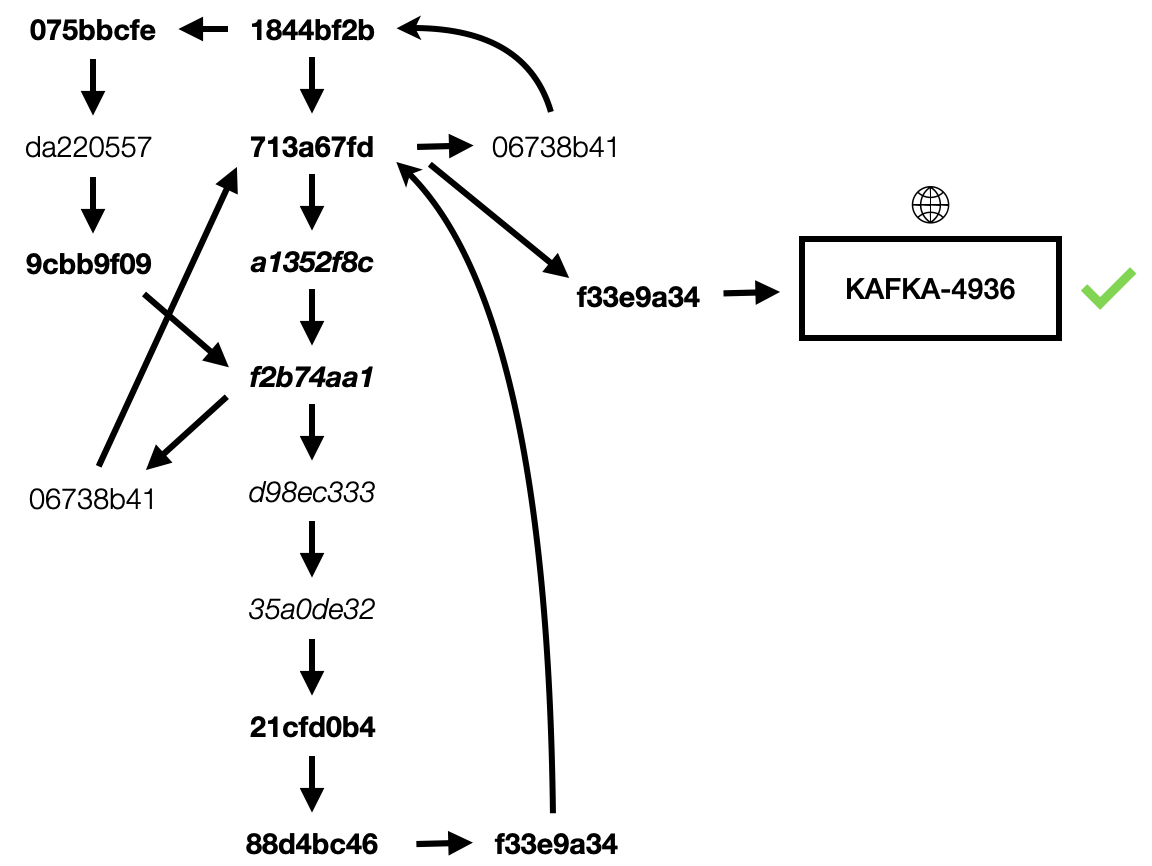
\includegraphics[width=12cm]{./images/graph-sample-A.png}}}%
  \qquad
  \subfloat[\centering \participant{H}'s commit history exploration in answering question B1 without Intelligent History. 
    \label{subfig:Exploration-Graph-B}]{{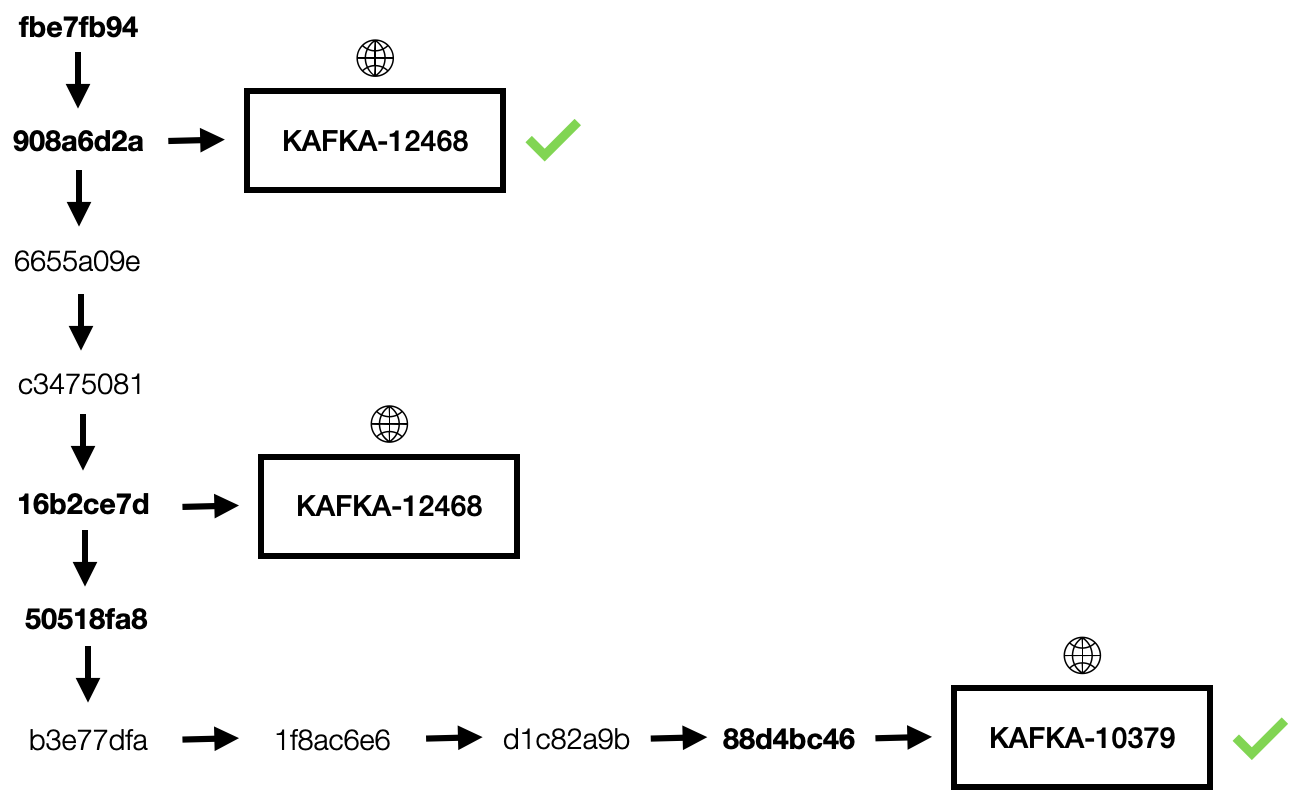
\includegraphics[width=12cm]{./images/graph-sample-B.png}}}%
  \caption{
    Commit history exploration graphs.
  }%
  \label{fig:Exploration-Graphs}%
\end{figure}

We determine a participant's commit history exploration approach based on the structure 
of the participant's commit history exploration graphs and from reviewing the session recordings.
A participant's exploration approach is categorized as one of:
\textit{linear}, \textit{cyclic and backtracking}, or \textit{commit message skimming}.
We define \textit{linear} for directed graphs in which all of the nodes represent commits 
that were examined in chronological order by timestamp. 
We use \textit{cyclic and backtracking} to describe directed graphs 
containing at least two cycles, indicating that the participant has backtracked to
an earlier seen commit at least twice, causing a cycle. 
Lastly, \textit{commit message skimming} characterizes graphs where 
at least a third of the nodes are italicized commit hashes to indicate
that the commit messages were only glanced at by the participant but the
contents of the commit were not further inspected by the participant.
If the condition for a graph to be categorized as \textit{commit message skimming} is met,
we categorize the graph as such regardless of whether the graph meets the critiera for the other two categories.

The complete set of commit history exploration graphs we constructed
for each participant is available in a public repository.\footnote{\url{https://github.com/Alison-Li/ubcthesis-dataset}, verified 7/25/2022.}
For each participant, we use the commit history exploration graph for question B1
as a starting point to characterize the participant's exploration approach since
B1 requires interaction with the larger commit history of the two files the participants were asked to explore.
B1 is also only answerable by considering several commits in the commit history since the
participant must make sure that the commits they select to use in their answer meet the conditions specified in the question.
For cases where a participant's graph for B1 may fit into more than one category for a commit history exploration approach,
we used the participant's graphs for A1, A2, and B2 to determine the dominant structure we observed across all graphs.

As a demonstration of how we devised categories for the participants' exhibited approaches for commit history exploration, 
\autoref{subfig:Exploration-Graph-A} illustrates participant \participant{B}'s approach to finding 
two meaningful commits as per question B1 without using Intelligent History.
The commit history exploration graph for \participant{B} shows they examined 16 out of 45 commits.
Participant \participant{B} would examine a few commits at a time,
as seen by the long linear series of commits explored in the left side of \autoref{subfig:Exploration-Graph-A}.
Participant \participant{B} then backtracked to previously seen commits 
after gaining a broad sense of the changes made over time to the file,
as seen by the jumps between \commit{059a81e3} back to the beginning of their search at \commit{fbe7fb94}, 
then to later to \commit{88d4bc46} and back to \commit{908a6d2a}.
We characterize the structure of the graph for \participant{B} as \textit{cyclic and backtracking},
given the three cycles in the graph we observed.

Meanwhile, the commit history graph for \participant{H} shown in \autoref{subfig:Exploration-Graph-B}, 
who answered the same question without Intelligent History, shows they examined 10 out of 45 commits.
Participant \participant{H} systematically examined 
each commit sequentially in chronological order by each commit's timestamp.
We characterize the structure of the graph for \participant{H} and their commit history exploration approach as \textit{linear} 
to describe the participant's sequential exploration of the commit history.

To analyze the participants' responses to the open-ended interview questions, 
we categorize each participant's experience with looking at issues and commits,
the commit history exploration approach they exhibitied when searching for the answers to the question sets, 
and the features of Intelligent History for which they expressed the most enthusiasm.
In the interviews, we asked participants how often they looked at commits and issues 
and categorized their responses as: 
\textit{often}, \textit{sometimes}, or \textit{rarely}.
We determined the feature of Intelligent History that a particiant found most favourable from
(\feature{1}) \textit{Highlight Important Changes}, 
(\feature{2}) \textit{Show Diff Metadata}, and
(\feature{3}) \textit{Show Jira Metadata}
based on a trend we observed in the participants' responses to interview question (4) from \autoref{fig:Interview-Questions}.
When interviewed about comparing their experience with and without using Intelligent History,
participants typically stated the feature of Intelligent History to which they responded most positively.
We also create a flowchart to illustrate and observe if there is any 
relationship between these categories for each participants.

%%%%%%%%%%%%%%%%%%%%%%%%%%%%%%%%%%%%%%%%%%%%%%%%%%%%%%%%%%%%%%%%%%%%%%
\section{Results}
\label{sec:Results}

\subsection{RQ1}
\label{subsec:RQ1}

\RQ{1}{\rev{Does Intelligent History accurately identify the commits that software developers want to examine?}}

We summarize the quantitative results collected through logs and screen recordings in \autoref{tab:Results-Quantitative-AB} 
for participants who received question set A first, then set B.
Likewise, the results for participants who received question set B first, then set A are summarized in \autoref{tab:Results-Quantitative-BA}.
In addition to the total number and proportion of unique commits a participant examined as part of answering a question,
we computed the proportion of those commits that would be highlighted commits according to Intelligent History.
We did this to observe:
(1) whether a large proportion of commits a participant inspects would be considered as important using Intelligent History
and (2) the influence of Intelligent History's commit highlighting on which commits a participant chooses to examine.

%% BEGIN: Large landscape tables
\begin{landscape}
  \begin{table}
    \caption{
      Summary of results for participants who received question set A first to complete without the plugin and question set B after to complete with the plugin.
      For each question set and question, the table shows the percentage of commits from the commit history that the participant examined (\%CE), 
      the percentage of the participant's examined commits that would be or were highlighted by the plugin (\%HC),
      the number of application switches between the \entity{IDE} and the browser (\#AC) that the participant made,
      and the number of Jira issues the participant viewed or accessed (\#IV).
    }
    \centering
    \resizebox{\columnwidth}{!}{%
      \begin{tabular}{@{}crrrrrrrrrrrrrrrr@{}}
        \toprule
        \multicolumn{1}{l}{}                & \multicolumn{8}{c}{Set A (without plugin)}                                                                                                                            & \multicolumn{8}{c}{Set B (with plugin)}                                                                                                                                                                 \\ \midrule
        \multicolumn{1}{c|}{}               & \multicolumn{4}{c|}{A1}                                  & \multicolumn{4}{c|}{A2}                                                                                    & \multicolumn{4}{c|}{B1}                                                                     & \multicolumn{4}{c}{B2}                                                                                    \\ \midrule
        \multicolumn{1}{c|}{Pseudo-initial} & \%CE      & \%HC      & \#AS & \multicolumn{1}{l|}{\#IV} & \multicolumn{1}{l}{\%CE} & \multicolumn{1}{l}{\%HC} & \multicolumn{1}{l}{\#AS} & \multicolumn{1}{l|}{\#IV} & \%CE      & \multicolumn{1}{l}{\%HC} & \multicolumn{1}{l}{\#AS} & \multicolumn{1}{l|}{\#IV} & \multicolumn{1}{l}{\%CE} & \multicolumn{1}{l}{\%HC} & \multicolumn{1}{l}{\#AS} & \multicolumn{1}{l}{\#IV} \\ \midrule
        \multicolumn{1}{c|}{A}              & 40.9 (9)  & 55.6 (5)  & 1.0  & \multicolumn{1}{c|}{1}    & 27.3 (6)                 & 83.3 (5)                 & 1.0                      & \multicolumn{1}{c|}{1}    & 15.6 (7)  & 100.0 (7)                & 0.0                      & \multicolumn{1}{c|}{4}    & 6.7 (3)                  & 100.0 (3)                & 0.0                      & 1                        \\
        \multicolumn{1}{c|}{C}              & 4.5 (1)   & 100.0 (1) & 1.0  & \multicolumn{1}{c|}{1}    & 27.3 (6)                 & 83.3 (5)                 & 1.0                      & \multicolumn{1}{c|}{1}    & 6.7 (3)   & 100.0 (3)                & 0.0                      & \multicolumn{1}{c|}{2}    & 0.0 (0)                  & N/A                      & 0.0                      & 0                        \\
        \multicolumn{1}{c|}{E}              & 36.3 (8)  & 62.5 (5)  & 1.0  & \multicolumn{1}{c|}{1}    & 68.1 (15)                & 66.7 (10)                & 1.0                      & \multicolumn{1}{c|}{1}    & 35.6 (16) & 100.0 (16)               & 1.0                      & \multicolumn{1}{c|}{3}    & 8.9 (4)                  & 100.0 (4)                & 0.0                      & 1                        \\
        \multicolumn{1}{c|}{G}              & 86.3 (19) & 57.9 (11) & 1.0  & \multicolumn{1}{c|}{1}    & 36.3 (8)                 & 75.0 (6)                 & 1.0                      & \multicolumn{1}{c|}{1}    & 13.3 (6)  & 100.0 (6)                & 3.0                      & \multicolumn{1}{c|}{5}    & 6.7 (3)                  & 100.0 (3)                & 1.0                      & 2                        \\
        \multicolumn{1}{c|}{I}              & 4.5 (1)   & 83.3 (5)  & 1.0  & \multicolumn{1}{c|}{1}    & 36.3 (8)                 & 75.0 (6)                 & 1.0                      & \multicolumn{1}{c|}{1}    & 6.7 (3)   & 100.0 (3)                & 0.0                      & \multicolumn{1}{c|}{2}    & 6.7 (3)                  & 100.0 (3)                & 0.0                      & 1                        \\ \midrule
        \multicolumn{1}{l|}{Mean}           & 34.5      & 68.5      & 1.0  & \multicolumn{1}{c|}{1}    & 39.1                     & 76.7                     & 1.0                      & \multicolumn{1}{c|}{1}    & 15.6      & 100.0                    & 0.8                      & \multicolumn{1}{c|}{3.2}  & 5.8                      & 100.0                    & 0.2                      & 1                        \\
        \multicolumn{1}{l|}{Median}         & 36.3      & 62.5      & 1.0  & \multicolumn{1}{c|}{1}    & 36.3                     & 75.0                     & 1.0                      & \multicolumn{1}{c|}{1}    & 13.3      & 100.0                    & 0.0                      & \multicolumn{1}{c|}{3.0}  & 6.7                      & 100.0                    & 0.0                      & 1                        \\ \bottomrule
      \end{tabular}
    }%
    \label{tab:Results-Quantitative-AB}
  \end{table}
\end{landscape}

\begin{landscape}
  \begin{table}
    \caption{
      Summary of results for participants who received question set B first to complete without the plugin and question set A after to complete with permitted use of the plugin.
      The same columns as shown in \autoref{tab:Results-Quantitative-AB} are used.
    }
    \centering
    \resizebox{\columnwidth}{!}{%
      \begin{tabular}{@{}crrrrrrrrrrrrrrrr@{}}
        \toprule
        \multicolumn{1}{l}{}                & \multicolumn{8}{c}{Set A (with plugin)}                                                                                                                              & \multicolumn{8}{c}{Set B (without plugin)}                                                                                                                                                              \\ \midrule
        \multicolumn{1}{c|}{}               & \multicolumn{4}{c|}{A1}                                 & \multicolumn{4}{c|}{A2}                                                                                    & \multicolumn{4}{c|}{B1}                                                                     & \multicolumn{4}{c}{B2}                                                                                    \\ \midrule
        \multicolumn{1}{c|}{Pseudo-initial} & \%CE     & \%HC      & \#AS & \multicolumn{1}{l|}{\#IV} & \multicolumn{1}{l}{\%CE} & \multicolumn{1}{l}{\%HC} & \multicolumn{1}{l}{\#AS} & \multicolumn{1}{l|}{\#IV} & \%CE      & \multicolumn{1}{l}{\%HC} & \multicolumn{1}{l}{\#AS} & \multicolumn{1}{l|}{\#IV} & \multicolumn{1}{l}{\%CE} & \multicolumn{1}{l}{\%HC} & \multicolumn{1}{l}{\#AS} & \multicolumn{1}{l}{\#IV} \\ \midrule
        \multicolumn{1}{c|}{B}              & 4.5 (1)  & 100.0 (1) & 1.0  & \multicolumn{1}{c|}{1}    & 9.0 (2)                  & 100.0 (2)                & 0.0                      & \multicolumn{1}{c|}{1}    & 35.6 (16) & 37.5 (6)                 & 2.0                      & \multicolumn{1}{c|}{2}    & 4.4 (2)                  & 100.0 (1)                & 0.0                      & 0                        \\
        \multicolumn{1}{c|}{D}              & 31.8 (7) & 100.0 (1) & 1.0  & \multicolumn{1}{c|}{1}    & 13.3 (6)                 & 100.0 (1)                & 1.0                      & \multicolumn{1}{c|}{1}    & 20.0 (9)  & 55.6 (5)                 & 2.0                      & \multicolumn{1}{c|}{2}    & 8.9 (4)                  & 100.0 (4)                & 2.0                      & 2                        \\
        \multicolumn{1}{c|}{F}              & 4.5 (1)  & 100.0 (1) & 1.0  & \multicolumn{1}{c|}{1}    & 13.6 (3)                 & 100.0 (3)                & 1.0                      & \multicolumn{1}{c|}{1}    & 42.2 (19) & 42.1 (8)                 & 1.0                      & \multicolumn{1}{c|}{1}    & 2.2 (1)                  & 100.0 (1)                & 1.0                      & 1                        \\
        \multicolumn{1}{c|}{H}              & 4.5 (1)  & 100.0 (1) & 1.0  & \multicolumn{1}{c|}{1}    & 31.8 (7)                 & 85.7 (6)                 & 1.0                      & \multicolumn{1}{c|}{1}    & 22.2 (10) & 50.0 (5)                 & 3.0                      & \multicolumn{1}{c|}{3}    & 8.9 (4)                  & 100.0 (4)                & 1.0                      & 1                        \\
        \multicolumn{1}{c|}{J}              & 4.5 (1)  & 100.0 (1) & 1.0  & \multicolumn{1}{c|}{1}    & 31.8 (7)                 & 100.0 (7)                & 0.0                      & \multicolumn{1}{c|}{1}    & 46.7 (21) & 71.4 (15)                & 2.0                      & \multicolumn{1}{c|}{2}    & 6.7 (3)                  & 100.0 (3)                & 1.0                      & 1                        \\ \midrule
        \multicolumn{1}{l|}{Mean}           & 10.0     & 100.0     & 1.0  & \multicolumn{1}{c|}{1}    & 19.9                     & 97.1                     & 0.6                      & \multicolumn{1}{c|}{1}    & 33.3      & 51.3                     & 2.0                      & \multicolumn{1}{c|}{2}    & 6.2                      & 100.0                    & 1.0                      & 1                        \\
        \multicolumn{1}{l|}{Median}         & 4.5      & 100.0     & 1.0  & \multicolumn{1}{c|}{1}    & 13.6                     & 100.0                    & 1.0                      & \multicolumn{1}{c|}{1}    & 35.6      & 50.0                     & 2.0                      & \multicolumn{1}{c|}{2}    & 6.7                      & 100.0                    & 1.0                      & 1                        \\ \bottomrule
      \end{tabular}
    }%
    \label{tab:Results-Quantitative-BA}
  \end{table}
\end{landscape}
%% END: Large landscape tables

We found for questions that participants completed without Intelligent History,
over half of the commits that participants examined would have been highlighted by Intelligent History.
For A1 and A2 respectively, a mean of 68.5\% and 76.7\% 
of the commits that the participants examined would be highlighted commits (see \autoref{tab:Results-Quantitative-AB}).
For B1 and B2 respectively, a mean of 51.3\% and 100.0\% 
of the commits that the participants examined would be highlighted commits (see \autoref{tab:Results-Quantitative-BA}).
This indicates that in cases where Intelligent History is not used and therefore does not influence the commits participants examine,
we observe a degree of overlap between the commits that participants choose to further investigate and the commits that Intelligent History highlights.

When participants had access to Intelligent History,
nearly 100.0\% of the commits they examined for a question were highlighted commits.
For A1, a mean of 100.0\% of the commits that particpants who used Intelligent History examined were highlighted commits (see \autoref{tab:Results-Quantitative-BA}).
For A2, the mean was 97.1\% of the commits (see \autoref{tab:Results-Quantitative-BA}).
Similarly for B1 and B2, a mean of 100.0\% of the commits that participants who used Intelligent History examined were highlighted commits (see \autoref{tab:Results-Quantitative-AB}).
According to these results, we make the observation that highlighted commits heavily 
influenced how participants selected commits from the commit history for further investigation, as
nearly all of the commits that participants chose to inspect from the commit history were commits that Intelligent History highlighted.
While this is not sufficient evidence to comment about the agreement from participants on the commits Intelligent History
chooses to highlight and not highlight,
we observe that participants did not choose to examine the commits Intelligent History did not highlight
for 3 out of 4 questions asked in the experiment.

In the interviews we conducted, 
several participants commented on how commit highlightling de-emphasized ``minor'' changes from the history \participants{BDEFH}.
Although participants were not asked to validate the commits that Intelligent History chose to highlight and to fade out from the commit history, 
participant \participant{B} expressed agreement with the highlighting, 
noting that the faded commits ``\textit{do not seem to be useful for this file [the \class{Topology} class] at all}.''

Overall, we find that these results to demonstrate how well the underlying approach of using regular expression
patterns for identifying less important changes in diffs show some promise as, on average,
at least half of the commits that participants examined for each question without Intelligent History
would be highlighted commits if they had used Intelligent History.
This represents an overlap of at least half of the commits that participants examined and the commits
that Intelligent History would highlight to indicate a potentially interesting commit.

\begin{summary}[RQ1]
  An implementation that uses a minimal set of regular expression patterns 
  applied to commit diffs to identify commits containing solely non-essential changes can help to
  automatically distinguish at least half of the commits that software
  developers want to examine.
\end{summary}

%%%%%%%%%%%%%%%%%%%%%%%%%%%%%%%%%%%%%%%%%%%%%%%%%%%%%%%%%%%%%%%%%%%%%%

\subsection{RQ2}
\label{subsec:RQ2}

\RQ{2}{Does highlighting important commits help software developers explore a file’s revision history more efficiently?}

We define our measure for efficiency as the proportion of commits from a file's commit history 
that a developer examines before \rev{providing a sufficient answer to} questions about the intent behind code changes.
From \autoref{tab:Results-Quantitative-AB} and \autoref{tab:Results-Quantitative-BA}, 
we observe that participants who did not use Intelligent History 
examined a higher mean proportion of commits for questions A1, A2, and B1.
The results of the $t$-tests for determining significant statistical differences in 
the mean proportion of commits examined by each group for a question are summarized in \autoref{tab:t-test}.

For questions A1 and B2, we fail to reject the null hypothesis, which states that the mean proportion of commits examined 
by the group without Intelligent History and the group with Intelligent History are equal.
However, for questions A2 and B1, we reject the null hypothesis, indicating the mean proportion of commits examined 
by the group without Intelligent History and the group without Intelligent History are not equal.
Thus, our findings show there is a significant difference in the mean proportion of commits examined between 
the group that does not use Intelligent History and the group that does use Intelligent History to answer questions A2 and B1.
We found that the results of the $t$-tests could be impacted by the differing natures between questions A1, A2 and B1, B2.
A2 and B1 are concerned with navigating a broad commit history and using the components of a commit, such
as the diff, messages, and issues, to identify whether a commit meets the conditions of a question.
A1 and B2 are related to locating the information for specific fragments of code,
where the commits affecting the section can be located without Intelligent History. 

\begin{table}[h]
  \caption{
    Results of single-tailed, two-sample $t$-tests at $\alpha = 0.05$ and $df = 8$ to determine if there is a significant difference between the proportion of commits examined from a commit history
    with and without Intelligent History.
  }
  \centering
  \begin{tabular}{@{}ccccc@{}}
    \toprule
    Set                                     & Question               & \multicolumn{1}{c}{$t$-value} & \multicolumn{1}{c}{$p$-value} & $H_{0}$ \\ \midrule
    \multicolumn{1}{c|}{\multirow{2}{*}{A}} & \multicolumn{1}{c|}{A1} & 1.53                        & 0.08                        & Fail to reject   \\ \cmidrule(l){2-5} 
    \multicolumn{1}{c|}{}                   & \multicolumn{1}{c|}{A2} & 2.13                        & 0.03                        & Reject   \\ \midrule
    \multicolumn{1}{c|}{\multirow{2}{*}{B}} & \multicolumn{1}{c|}{B1} & 2.37                        & 0.02                        & Reject   \\ \cmidrule(l){2-5} 
    \multicolumn{1}{c|}{}                   & \multicolumn{1}{c|}{B2} & -0.66                       & 0.26                        & Fail to reject   \\ \bottomrule
  \end{tabular}
  \label{tab:t-test}
\end{table}

\subsubsection{Navigating a Broad Commit History}

We observe that a possible explanation for the outcome of the $t$-tests on A2 and B1 are
because A2 and B1 require the participant to make full use of all the sources of
information they have in the commit history, which include the diffs, commit messages,
and any referenced Jira issues.
The participant must first examine the diffs to determine \rev{whether} the source code change
complies with what is asked in A2 and B1.
Since many commit messages are empty or brief, the participant is encouraged to view
the associated Jira issue to obtain the rationale information behind the code change.
As we observed in answering \entity{RQ1} (see \autoref{subsec:RQ1}), 
participants who had access to Intelligent History for a question
were more inclined to only examine highlighted commits.
Hence, participants answering questions with Intelligent History may have examined less commits
participants used highlighted commits as a way of prioritizing which commits to investigate further.

For question A2, participants who used Intelligent History examined a mean of 19.9\% of the commit history for the \class{Topology} class (see \autoref{tab:Results-Quantitative-BA}),
while participants who did not use Intelligent History examined a mean of 39.1\% of the same commit history (see \autoref{tab:Results-Quantitative-AB}). 
Interestingly, all of the participants who used Intelligent History to answer question set A 
responded most positively to feature (\feature{1}) \textit{Highlight Important Changes} from Intelligent History \participants{BDFHJ} 
(see \autoref{tab:Participants} and \autoref{tab:Flow-Chart-Tabular}).
This could have been because the group of participants who answered question set B first without Intelligent History 
and question set A after with Intelligent History were to reflect on how Intelligent History 
could have been useful for the question which they did not use Intelligent History with.

\rev{However, among participants who used Intelligent History to answer question set B,
4 out of 5 particiapnts demonstrated the most enthusiasm for (\feature{3}) \textit{Show Jira Metadata} instead \participants{ACGI},
while 1 participant preferred (\feature{1}) \textit{Show Jira Metadata} \participants{E}.
For the majority of participants who used Intelligent History with set B, this result may be due
to feature (\feature{3}) enabling participants to view larger mean number of issues for question B1 than the 
group who did not use Intelligent History for the same question (3.2 and 2).
Specifically for B1, which we expect to require accessing more Jira issues in order to be able
to understand the changes in many commits which can be vague, empty, or limited to explaining
what changed in the source code rather than why, the majority of participants who used Intelligent History
with B1, or set B overall, might have been more partial to (\feature{3}) since the questions
lead to more invocations of the feature.}

Participants generally commented on the utility of commit history highlighting for focusing their attention on commits that were highlighted 
and ignoring non-highlighted commits, which they regarded as ``irrelevant'' or ``minor'' \participants{BF}.
Participant \participant{B} said:

\begin{quote}
  When I think to what I have to do at work, 
  often you don’t know what kind of modification you’re looking for. 
  Especially when automated tests break or something, 
  you’re going to be looking for something that is very recent and if you’re on a popular file, 
  there might be a lot of commits. 
  But with this [commit history highlighting], 
  you’d be able to easily filter out things that actually made differences rather than negligible changes.
\end{quote}

Specifically regarding answering A2, participant \participant{H} stated:

\begin{quote}
  [Highlighting commits] was amazing for speeding up what I had to search for. 
  Especially in finding that sink issue [in A2], if I didn’t have the pencil 
  [(\feature{1}) \textit{Highlight Important Changes}], 
  I think I would have gone through all the commits backwards and just try to see what the diffs are 
  but it removed a bunch of the ones that it [Intelligent History] deemed not useful 
  and it ended up being correct so I just skipped over a bunch [of commits].
\end{quote}

Comparing their experiences for answering the question set without and with Intelligent History, 
participants commented on the effect of commit history highlighting making commit history exploration faster by reducing the amount of irrelevant commits they would have examined \participants{DFHJ}.
Participant \participant{D} mentioned: 
``\textit{[The highlighting] allowed for me to skim through the necessary commits a lot quicker \dots 
and visually reduces the amount of clutter I had to look at.}''
In a similar vein, participant \participant{J} commented:
``\textit{[The highlighting] removed the obvious minor changes that I didn’t really need to look at.}''

Meanwhile, in answering question B1, participants who used Intelligent History 
examined a mean of 15.6\% of the commit history for the \class{StreamsBuilder} class (see \autoref{tab:Results-Quantitative-AB}),
whereas participants who did not use Intelligent History examined a mean of 33.3\% of the same 
commit history (see \autoref{tab:Results-Quantitative-BA}).
Question B1 \rev{required} the participants to examine commits and diffs in the \class{StreamsBuilder} commit history 
to try to identify meaningful source code changes that were made to the class.
We clarified a meaningful source code change to be a commit that improves some functionality 
or behaviour in the class and expected participants to utilize the diffs and intent of a change's author to justify their answer.
Despite the group of participants who used Intelligent History to answer B2 looking at less than half the 
proportion of commits that the group who did not use Intelligent History looked at (15.6\% compared to 33.3\%),
only 1 participant emphasized commit history highlighting as a feature that made the strongest impression on them \participants{E}, 
whereas the remaining 4 participants showed a preference for feature 
(\feature{3}) \textit{Show Jira Metadata} of Intelligent History instead \participants{ACGI}.
Participant \participant{E} said:

\begin{quote}
  I think that the biggest benefit [of Intelligent History] was especially removing minor changes. 
  It’s [the \textit{Highlight Important Changes} feature] really handy; it filters a bunch of -- not garbage -- but noise in the commit history. 
  With just this single feature [commit history highlighting], it’s already worth using the plugin.
\end{quote}

On the commit history highlighting feature, participant \participant{A} stated:

\begin{quote}
  I liked the highlighting. 
  It’s nice to not look at so many commits. 
  [\dots] Looking at the history without the highlighting is kind of overwhelming because it’s just like ``oh my god, this is a flood of commits, 
  what are we going to do?'' 
  but when you get rid of the less important ones, it’s [\dots] much more manageable.
\end{quote}

Of the 6 participants that expressed a preference for feature (\feature{1}), 
2 employed a commit history exploration approach that could be described as \textit{cyclic and backtracking} based on their commit history exploration graphs \participants{BF},
3 used commit message skimming \participants{DJ}, and 1 used a linear approach \participants{H}.
Thus, we find there to be less of a relationship between a participant's software history exploration approach 
and their preference for feature (\feature{1}).

\subsubsection{Locating Rationale for a Code Fragment}

As captured from the results of the $t$-tests in \autoref{tab:t-test}, 
there was insufficient evidence from our study to support the claim of a significant difference in 
the proportion of commits examined by the groups for answering questions A1 and B2.
We observe this outcome may be attributed to the nature of both questions A1 and B2, 
which are similar as they require the participant to  inspect a specific section of code 
given by line numbers and attempt to locate commits relevant to these code segments.
As A1 and B2 are concerned with finding the intent behind certain code fragments, 
the commits that affect these code fragments can be narrowed down
through familiar features in IntelliJ such as the ``Show History for Selection'' feature 
that operates similarly to \entity{git} ``blame.''
Participants who vocalized familiarity with using \entity{git} ``blame'' and commented on typically
using the ``blame'' tool in Git were shown and permitted to use the native 
``Show History for Selection'' feature in IntelliJ feature, 
which enabled participants to view a subset of commits affecting selected fragments of source code.

In recognition of the suitability of commit history highlighting for certain types of questions,
2 participants who received question set B first without Intelligent History and question set A 
after with Intelligent History commented on their desire to use Intelligent History's commit highlighting feature for question B1
if they were to re-do the question because B1 required exploration of a larger commit history \participants{BD}.
Participant \participant{B} mentioned:

\begin{quote}
  [For] the questions [I was] asked [\dots] the plugin didn’t help that much. 
  For example, one of the questions in the \class{StreamsBuilder} class was to look for commits that improve things, 
  so I feel like if I had to re-do that task, then using the highlighting would have been useful.
\end{quote}

For question A1, 6 participants used the ``Show History for Selection'' feature \participants{CEFHIJ},
and the other 4 participants manually found the commit that introduced the change and contained the rationale information by reading the commit mesage subjects and using the chronological information based on other commit timestamps \participants{ABDG}.
For question B2, the failure to reject the null hypothesis may be attributed to the fact that the commit \commit{e09d6d79} which contains the information necessary for answering this question has the message title: 

\begin{center}
  \jira{KAFKA-7027:}{Add overloaded build method to StreamsBuilder (\#5437)} 
\end{center}

Hence, participants familiar with using version control tools for similar questions encountered 
in every day work would be able to quickly narrow down the commit needed to answer 
the question without requiring traversal of the file's commit history.
Due to the nature of A1 and B2 and the limited impact of commit highlighting 
on the participants' experience with answering these questions,
our samples are insufficient for obtaining evidence to show a significant difference in 
commit history exploration efficiency between the group that does not use Intelligent History 
and the group that does use Intelligent History for questions that ask about specific sections of code from a Java class.

Thus, based on our analysis of A2 and B1 where there was a significant difference in 
the proportion of commits examined by participants using Intelligent History, 
we observe that participants who use Intelligent History with its commit highlighting feature 
look at a smaller proportion of commits from a file's commit history when answering questions related to
identifying and finding meaningful source code changes over a general view of the commit history.
In support of this observation, 
participant \participant{A} expressed a beneficial use case of commit history highlighting 
for reducing the number commits a software developer examines:

\begin{quote}
  If I was trying to get a sense of major changes in a file, like say there was an issue that came up in a file and I’m looking for where it could have gotten introduced, 
  then that [highlighting commits] would be very useful because it gets rid of all the changes that don’t matter. 
\end{quote}

We found highlighting has the ability to distinguish non-essential commits from other commits in a commit history
for questions A2 and B1.
This is accompanied by a reduced percentage of commits examined when exploring a file's commit history 
for questions related to identifying meaningful source changes 
and the intent behind those changes when the developer must navigate a broad commit history for a file. 
For questions A1 and B2, which relate to finding the intent behind fragments of source code,
we have insufficient evidence to show that there is a significant difference
between the participant group that had highlighted commits and the group that did not have highlighted commits.

\begin{summary}[RQ2]
  Commit history highlighting can support software developers in efficiently 
  exploring commit history for code rationale information 
  by examining a smaller proportion of the commits in a file's commit history.
  Commit history highlighting makes identifying and searching for meaningful source code changes 
  across a broad commit history more efficient but has less impact when trying to find rationale information for specific code segments in a file.
\end{summary}

%%%%%%%%%%%%%%%%%%%%%%%%%%%%%%%%%%%%%%%%%%%%%%%%%%%%%%%%%%%%%%%%%%%%%%

\subsection{RQ3}
\label{subsec:RQ3}

\RQ{3}{How useful is direct integration of issue information in the IDE for helping a developer search for code rationale information?}

We found the utility of direct integration of issue information 
to be dependent on a participant's background with examing commits and issues,
and the software history exploration approach they employ.
The usefulness of direct integration of issue information is also dependent on 
\emph{what} information is extracted from an issue and \emph{how} it is presented in the \entity{IDE}.

\subsubsection{Developer Background and Exploration Approach}

We present a table in \autoref{tab:Flow-Chart-Tabular} to show the
categorization of each participant's background with regard to looking at commits
and issues, the commit history exploration strategy they exhibited as determined
using their commit history exploration graphs, and the feature of Intelligent History
to which they were most partial to.
The flowchart showing the relationship between each of these categories for each participant
is illustrated in \autoref{fig:Flow-Chart-Aggregate}.
Each participant tended to use the same commit history exploration strategy throughout the study, 
irrespective of the nature of the question asked and the presence of Intelligent History.
The features of Intelligent History are the actions we detailed in \autoref{sec:Implementation}, which are 
(\feature{1}) \textit{Highlight Important Changes}; 
(\feature{2}) \textit{Show Diff Metadata}; 
and (\feature{3}) \textit{Show Jira Metadata}.

\begin{table}
  \caption{
    The categorization of each participants' qualitative responses and their demonstrated commit history exploration approach.
    Favourable features of Intelligent History are indicated as:
    (\feature{1}) \textit{Highlight Important Changes},
    (\feature{2}) \textit{Show Diff Metadata}, and
    (\feature{3}) \textit{Show Jira Metadata}.
  }
  \centering
  \resizebox{\columnwidth}{!}{%
    \begin{tabular}{@{}c|ccc@{}}
      \toprule
      \textbf{Pseudo-initial} & \textbf{\begin{tabular}[c]{@{}c@{}}How often do you look\\ at commits and issues?\end{tabular}} & \textbf{\begin{tabular}[c]{@{}c@{}}Commit history\\ exploration approach\end{tabular}} & \multicolumn{1}{c}{\textbf{\begin{tabular}[c]{@{}c@{}}Favourable feature of\\ Intelligent History\end{tabular}}} \\ \midrule
      A                       & Sometimes                                                                                       & Cyclic and Backtracking                                                                & (\feature{3}) \\ \midrule
      B                       & Often                                                                                           & Cyclic and Backtracking                                                                & (\feature{1}) \\ \midrule
      C                       & Often                                                                                           & Linear                                                                                 & (\feature{3}) \\ \midrule
      D                       & Sometimes                                                                                       & Commit Message Skimming                                                                & (\feature{1}) \\ \midrule
      E                       & Rarely                                                                                          & Commit Message Skimming                                                                & (\feature{1}) \\ \midrule
      F                       & Often                                                                                           & Cyclic and Backtracking                                                                & (\feature{1}) \\ \midrule
      G                       & Sometimes                                                                                       & Cyclic and Backtracking                                                                & (\feature{3}) \\ \midrule
      H                       & Rarely                                                                                          & Linear                                                                                 & (\feature{1}) \\ \midrule
      I                       & Sometimes                                                                                       & Linear                                                                                 & (\feature{3}) \\ \midrule
      J                       & Rarely                                                                                          & Commit Message Skimming                                                                & (\feature{1}) \\ \bottomrule
    \end{tabular}
  }%
  \label{tab:Flow-Chart-Tabular}
\end{table}

\begin{figure}[h]
  \centering
  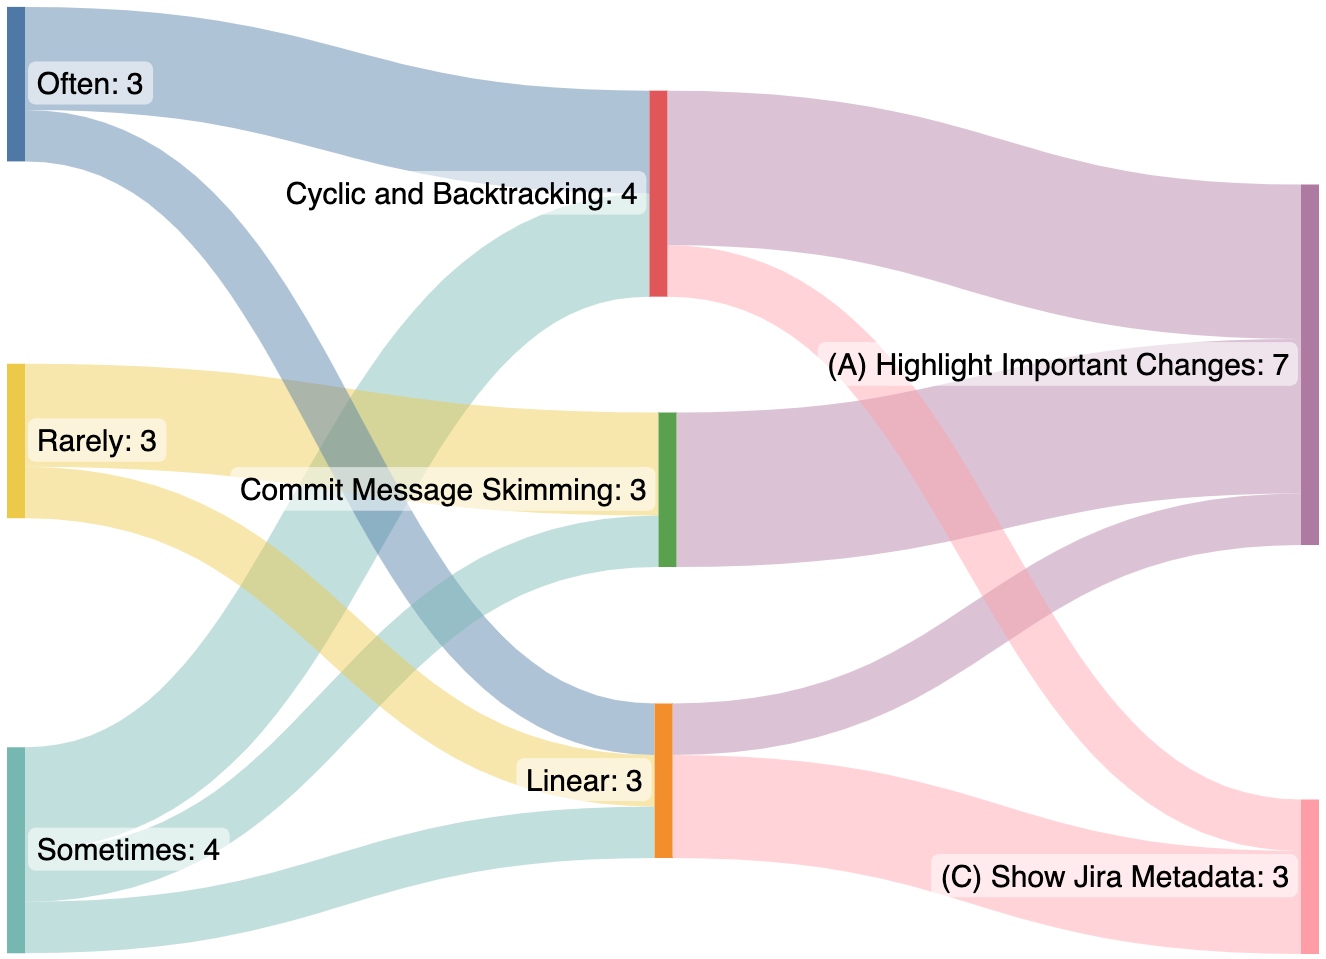
\includegraphics[width=8cm]{./images/flow-chart-aggr.png}
  \caption{
    An aggregated version of the data in \autoref{tab:Flow-Chart-Tabular}.
  }
  \label{fig:Flow-Chart-Aggregate}
\end{figure}

Over half of the participants, 6 out of 10, preferred feature (\feature{1}) from Intelligent History the most,
whereas the other 4 participants preferred feature (\feature{3}).
Notably, all 5 of the participants who received question set A to answer with Intelligent History 
responded most positively to commit history highlighting in (\feature{1}) as a feature \participants{BDFHJ}, 
whereas 4 out of the 5 participants who received question set B to answer with Intelligent History 
responded most positively to gaining quick access to Jira issue information within the \entity{IDE} in (\feature{3}) as a feature \participants{ACGI}.
This signifies some degree of correlation between the question set and the participants' most preferred features of Intelligent History.

None of the participants chose feature (\feature{2}), though we anticipated this outcome as (\feature{2}) 
was provided to give the user context as to how Intelligent History highlights commits in (\feature{1}).
Among the 3 participants who stated that they often look at commits and issues, none demonstrated \textit{commit message skimming} 
as a strategy for exploring commit history.
Similarly, of the 3 participants who rarely look at commits and issues, none employed a commit history exploration approach 
that we could characterize as \textit{cyclic and backtracking}.
There does not appear to be any concrete associations between how frequently a participant looks at commits and issues
and their exhibited approach to exploring commit history in our experiment.

On the relationship between the commit history exploration approach 
a participant exhibited and their preferred feature from Intelligent History,
we see that 2 out of 3 participants who exhibited a \textit{linear} strategy preferred feature (\feature{3}) \participants{CI},
while 1 favoured feature (\feature{1}) \participants{H}.
We observe that 2 out of 4 participants who demonstrated a \textit{cyclic and backtracking} 
approach expressed preference for (\feature{1}) \participants{BF},
while the other 2 participants favoured (\feature{3}) \participants{AG}.
None of the participants who exhibited a \textit{commit message skimming} strategy 
were most partial to (\feature{3}).

\subsubsection{Breadth and Contextualization}

We anticipated question B1 to require the most application switching between the \entity{IDE} 
and browser and to have the highest number of mean Jira issues viewed.
This is because B1 requires participants to examine the diffs of commits to ensure they consist of source code changes 
that comply with the criteria of improving some functionality or behaviour in the \class{StreamsBuilder} class.
Participants were also asked to justify their answer by finding supporting evidence for the commit author's intent behind their change.

The participant group who did not use Intelligent History with B1 had a mean number of application switches of 2.0 (see \autoref{tab:Results-Quantitative-BA}),
while the group who did use Intelligent History with B1 had a mean number of application switches of 0.8 (see \autoref{tab:Results-Quantitative-AB}).
The group who did not use Intelligent History with B1 viewed a mean of 2.0 Jira issues (see \autoref{tab:Results-Quantitative-BA}),
while the group who did use Intelligent History with B1 viewed a mean of 3.2 Jira issues (see \autoref{tab:Results-Quantitative-AB}).
We observe that participants who used Intelligent History for locating meaningful source code changes and finding the code rationale behind the changes
were able to view more Jira issues with slightly less application switches than participants who did not use Intelligent History for the same task.

Coincidentally, 4 of the 5 participants from the group that answered question set B with 
Intelligent History actually favoured feature (\feature{3}) \textit{Show Jira Metadata} \participants{ACGI}.
Participant \participant{A} commented:

\begin{quote}
  I thought that the Jira integration was very helpful because you don’t have to go to Jira to look at all the stuff and deal with Jira. 
  It’s [the issues] just in the \entity{IDE} which is nice; it’s [the plugin] quick and fast.
\end{quote}

Participant \participant{I} mentioned:

\begin{quote}
  Without the plugin, it was a little more annoying and time-consuming opening up the browser, 
  looking for all of the issues. 
  Whereas with the plugin, 
  it was already there [in the \entity{IDE}] and I can just take a quick look and see if it [the commit] 
  might be relevant and I can take a deeper look if needed.
\end{quote}

Among the 4 participants who favoured (\feature{3}), none demonstrated a 
\textit{commit message skimming} strategy to exploring commit history in the study.
As seen in \autoref{fig:Flow-Chart-Aggregate}, 2 of the participants exhibited 
a \textit{linear} approach \participants{CI}, 
while the other 2 participants exhibited a \textit{cyclic and backtracking} approach \participants{AG}.
Only 1 of the participants reported looking at commits and issues often \participants{C},
while 3 participants reported sometimes looking at commits and issues \participants{AGI}.
Unsurprisingly, all of the participants who favoured (\feature{3}) 
did not report to rarely looking at commits and issues.

While we observed that there was some notable difference in the group that used Intelligent History 
and the group that did not use Intelligent History for question B1,
there is less notable difference between the groups for question B2.
Hence, we find that the primary question responsible for this bias is question B1.
Given the nature of B1, we find direct integration of Jira issue information within the \entity{IDE} 
to be useful for broad search and exploration of a commit history.
As participant \participant{E} stated:
``\textit{[The Jira issue integration] helps you contextualize the code change in a commit really quick.}''
However, direct issue integration is potentially less useful for those with an approach based on skimming commit messages.

\subsubsection{Issue Content and Presentation}

We found 2 participants mentioned a preference to see the full Jira issue information contextualized in the browser interface \participants{DF}.
While participant \participant{F} explained that they were accustomed to viewing Jira issues in the browser,
participant \participant{D} stated that they had a preference to view all items associated with a Jira issue, including all linked issues and pull requests:
``\textit{When I’m looking at a Jira ticket, I look at everything associated with the ticket to try to get a much broader context.}''
On the other hand,
participant \participant{E} stated that they did not look at parts of an issue beyond the description and a few comments:
``\textit{I wouldn’t bother that much with looking at the issue for other things like discussion, other than the description and perhaps the last two comments, 
I wouldn’t look much further than that}.''
We found there may be some limitations related to \emph{what} information was presented in the integrated view of the Jira issue in the \entity{IDE}
and the personal preferences and habits of the user.

Similar in sentiment, participant \participant{G}, who favoured (\feature{3}), noted the hyperlinking of Jira issues for each commit
was most helpful to them in the study.
Participant \participant{G} observed that since some of the Jira issues 
included code fragments, it was difficult to read them in the \entity{IDE}.
This indicates the presentation of the issue information may be an impediment to its utility.

\begin{summary}[RQ3]
  Direct integration of issue information might better assist software developers 
  who use a \textit{linear} or \textit{cyclic and backtracking} approach to exploring commit history 
  in contextualizing source code changes and providing access to the information in more issues than without.
  However, the utility of direct integration of issue information is dependent on users' preferences 
  for \emph{what} content they wish to see from issues and \emph{how} they would like 
  the information to be presented.
\end{summary}

%%%%%%%%%%%%%%%%%%%%%%%%%%%%%%%%%%%%%%%%%%%%%%%%%%%%%%%%%%%%%%%%%%%%%%

\section{Threats to Validity}

\subsection{Construct Validity}

The size of the question sets we asked is a threat to construct validity.
Due to the laboratory setting of the study and the time estimated for participants to perform environment setup,
be introduced to the Apache Kafka project, Jira, the IntelliJ IDEA IDE, and the Intelligent History plugin,
we restricted the number of questions asked to account for a reasonable total estimated session time.
We formulated small sets of questions to relieve participants from a time limit 
and give them the freedom to explore the commit histories, inspect individual commits, and read Jira issues at their own pace.
Although the small quantity of questions allowed us to observe the participants closely for each information-finding question,
we risk the ability to observe the consistency of the participants' commit history exploration strategies
across larger sets of questions to use without and with Intelligent History.

The realism of the questions we asked also threatens construct validity.
The questions we formulated in A1, A2, B1, and B2 and the commit history exploration 
they require may not be reflective of the tasks software developers perform in practice.
\rev{For example, B1 asks a participant to search for and identify two meaningful commits from a 
file's commit history. However, participant \participant{A} noted they would typically
search for commits in relation to some event such as the occurrence of a bug and look
for commits that may have had a role in the introduction of such a bug.}
The questions from our experiment and the activities required to answer the questions would typically be
asked or performed in the context of \rev{task with a more concrete objective}, 
such as tracing the origin of a bug \rev{or, as participant \participant{F} mentioned, 
seeking the introduction of a specific feature to use as a model for developing a similar feature.}

\subsection{Internal Validity}

The presence of an observer in the experiment sessions means the participants' behaviour, opinions, 
and feedback about the Intelligent History plugin are subject to the Hawthorne effect,
which threatens internal validity.
The presence of an observer could have caused participants to deviate from their regular work habits 
as the participants might have formed an expectation about how to behave or explore the commit history.
We attempted to mitigate this effect by minimizing observer interjections during the sessions, 
though prior to the study, participants were encouraged to think aloud to describe their strategies 
to finding the information necessary to answer the questions.
We also provided participants with the opportunity to self-report, clarify their actions, 
and provide feedback on their experience with participating in the experiment during the interviews.

The introduction of the Intelligent History plugin to the participant could be a threat to internal validity.
After being introduced to the features of Intelligent History, 
the participant could be biased to use or conduct themselves in the study a certain way.
For example, toggling feature (\feature{1}) \textit{Highlight Important Changes} 
results in highlighting the commits in a commit history to distinguish less important commits from potentially more important commits.
If we initially introduced Intelligent History to a participant for their first question set,
and asked the participants to work on a second question set without Intelligent History,
they may have tried to answer the questions in the same way they would have if they had access to Intelligent History.
Consequently, in the semi-structured interview part of the study, 
participants may have felt biased to feel a certain way about the plugin.

We tried to avoid bias in how a participant expects to use Intelligent History 
and the utility of Intelligent History to a particular question set 
by alternating the order of the questions each participant received 
and fixing the use of the plugin to the second question set that each participant receives.
By providing each participant with a different set of questions to answer with 
and without Intelligent History respectively,
we also mitigate the threat to internal validity of a participant having 
exposure to the same questions prior to using Intelligent History.
Though the participants might have felt biased after using the plugin,
we would still be able to retain and collect data about how the participant approached 
exploring the commit history and answering the questions without being made aware of the plugin's features initially.

The experience of the participants with regard to having worked on a project that uses an issue tracking system 
and closely associating issues to commits impacts internal validity.
We tried to minimize the impact of a participant's background related 
to looking at commit and issues on internal validity by formulating questions 
that would require participants to justify their answers 
using source code and Jira issue information to encourage participants to view Jira issues.

\subsection{External Validity}

The sample size of 10 participants affects the generalizability of our results and is a threat to external validity.
Collecting data for a larger sample size may lead to more robust conclusions about the relationship 
between a developer's experience with looking at issues and commits,
the commit history exploration strategy or strategies they employ, 
and the aspects of Intelligent History they found to be most useful.
Nevertheless, a strength of our participant pool is representation. 
We obtained samples from 4 students and 6 professional developers from different companies,
representing a combination of participants from academia and industry.

A field study to investigate and evaluate the performance of the approaches in Intelligent History might also be needed to improve generalizability.
Rather than designing sets of questions pertaining to the commit history and issues available in one open-source repository,
which was Apache Kafka in our experiment,
a field study to investigate how developers explore commit history with and without Intelligent History in the wild 
could lead to a more robust model for determining non-essential and essential commits,
as well as gain a deeper understanding of how often developers use issues from an issue tracking system and how they prioritize the information in an issue.

%%%%%%%%%%%%%%%%%%%%%%%%%%%%%%%%%%%%%%%%%%%%%%%%%%%%%%%%%%%%%%%%%%%%%%
\endinput

Any text after an \endinput is ignored.
You could put scraps here or things in progress.